\documentclass{beamer}
\mode<presentation>
\usetheme{Berlin}
\usecolortheme{beaver}

%%%
% TITLE PREAMBLE
\title[Intro to Bioinformatics] % (optional, only for long titles)
{An Introduction to Bioinformatics Tools}
\subtitle{Basics of Robust and Repeatable Data Analysis}
\author[Pritchard, Cock] % (optional, for multiple authors)
{Leighton~Pritchard \and Peter~Cock}
\institute[The James Hutton Institute] % (optional)
{
  Information and Computational Sciences\\
  The James Hutton Institute
}
\date[May 2014] % (optional)
{Bioinformatics Training, 29$^{th}$ May 2014}
\subject{Bioinformatics}

%%%
% TOC
% Show table of contents, with current section highlighted,
% at the start of each section
\AtBeginSection[]
{
  \begin{frame}
    \frametitle{Table of Contents}
    \tableofcontents[currentsection]
  \end{frame}
}


%%%
% START DOCUMENT
\begin{document}

  \frame[plain]{\titlepage}

 %%%
 % SECTION: Introduction
  \section{Introduction}
  \begin{frame}
    \frametitle{Introduction}
    \framesubtitle{Course scope and limitations}
    \begin{itemize}
	\item<1-> Running programs is not doing bioinformatics
	\item<2-> appears from slide 2 on
	\item<3-> appears from slide 3 on
	\item<4-> appears from slide 4 on
	\end{itemize}
  \end{frame}

  \begin{frame}
    \frametitle{This is the second slide}
    \framesubtitle{A bit more information about this}
    %More content goes here
  \end{frame}

 %%%
 % SECTION: Recording your work
   \section{Recording Your Work}
   
   % SUBSECTION: justification
   \subsection{Why and How?}
   \begin{frame}
     \frametitle{Why Do It?}
     \begin{itemize}
	   \item Doing bioinformatics is doing science: keep a lab book!
	   \item Reproducibility
	   \item \textit{You will not remember} multiple files, databases, analysis details, etc.
	   \item Good advice: Noble (2009) \textit{PLoS Comput. Biol.} \url{http://dx.doi.org/10.1371/journal.pcbi.1000424}
	\end{itemize}
	
\includegraphics[width=.75\textwidth]{images/noble_2009_head}
   \end{frame}
   
   \begin{frame}
     \frametitle{How To Do It?}
     \begin{itemize}
	   \item There is no one correct way, but$\ldots$
	   \item Think about it \textit{before} you start
	   \item Use plain text where possible
	   \item Use version control
	   \item Keep backups
	   \item Different tools are suited to different purposes: code \textit{vs.} data \textit{vs.} analysis \textit{vs.} $\ldots$
	\end{itemize}
   \end{frame}
   
   \begin{frame}
     \frametitle{Where to get more advice?}
     \begin{itemize}
	   \item Ask us (we do this a lot)
	   \item BioStars (\url{https://www.biostars.org})
	   \item SeqAnswers (\url{http://seqanswers.com/})
	   \item \textit{PLoS Comp Biol} collections (\url{http://www.ploscollections.org/static/pcbiCollections})
	\end{itemize}
	
\includegraphics[width=.2\textwidth]{images/gibas_book}
	
\includegraphics[width=.2\textwidth]{images/buffalo_book}
   \end{frame}
   
   % SUBSECTION: useful tools
   \subsection{Useful Tools}
   \begin{frame}
     \frametitle{Plain Text Files}
     \begin{itemize}
       \item \texttt{README.txt}/\texttt{README.md} in each directory/folder
       \item Plain text = always human-readable
       \item Markdown (\url{https://daringfireball.net/projects/markdown/basics})
       \item RST (\url{http://docutils.sourceforge.net/docs/ref/rst/restructuredtext.html})
     \end{itemize}
    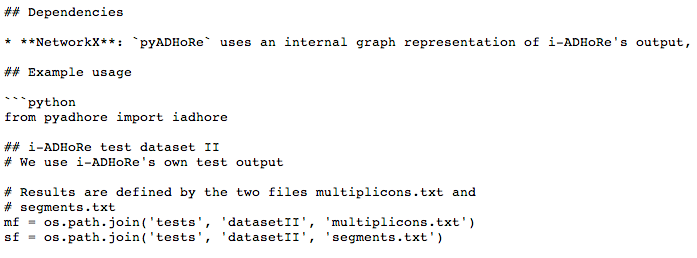
\includegraphics[width=.4\textwidth]{images/markdown_before}
	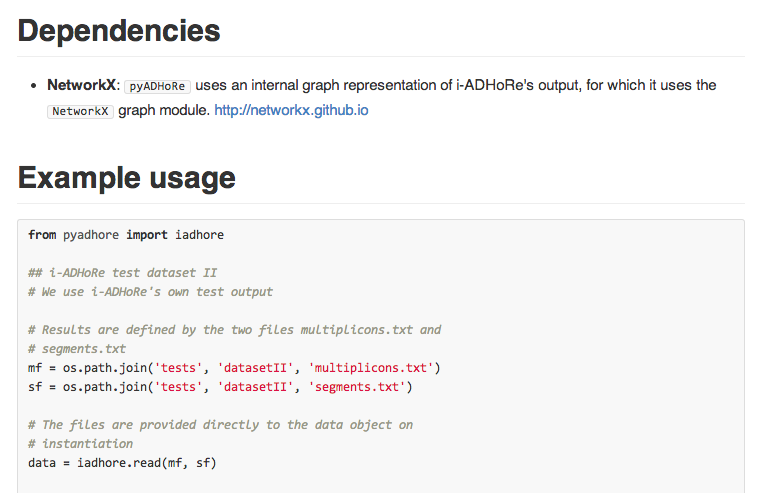
\includegraphics[width=.4\textwidth]{images/markdown_after}
   \end{frame}
   
   \begin{frame}
     \frametitle{\LaTeX}
     \begin{itemize}
       \item Powerful, versatile typesetting system
       \item Similar to markup/markdown
       \item Great for mathematical/computing work
     \end{itemize}
    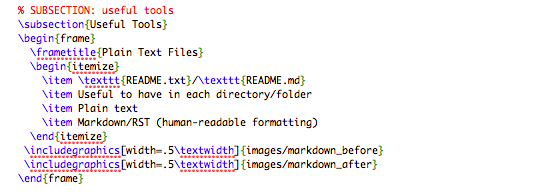
\includegraphics[width=.35\textwidth]{images/latex_before}
	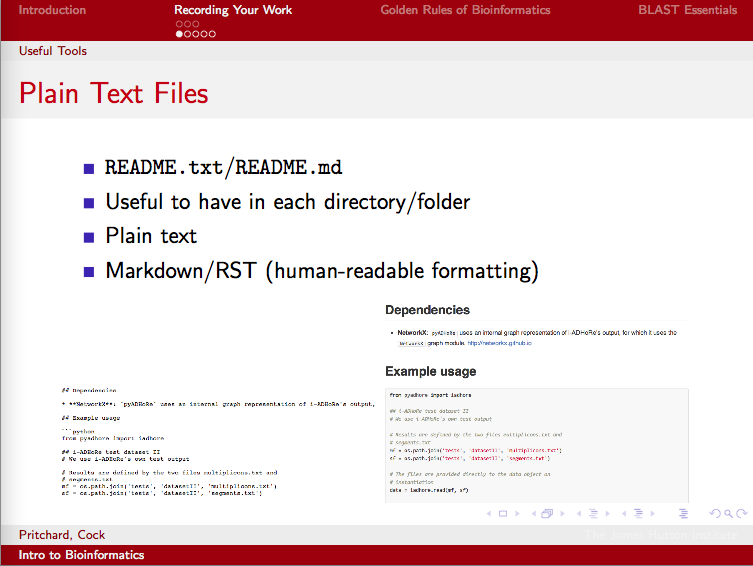
\includegraphics[width=.35\textwidth]{images/latex_after}     
   \end{frame}
   
   \begin{frame}
     \frametitle{\texttt{script}}
     \begin{itemize}
       \item use \texttt{man script} at your terminal
       \item Writes your terminal activity to a plain text file
       \item Saves effort copy/pasting and typing commands into a lab book, as you go
       \item Easy to use with other tools 
     \end{itemize}
   \end{frame}
   
   \begin{frame}
     \frametitle{Wiki}
     \begin{itemize}
       \item Useful for shared projects/data
       \item Automatic version control (and attribution)
     \end{itemize}
   \end{frame}
   
   \begin{frame}
     \frametitle{language notebook}
     \begin{itemize}
       \item e.g. \texttt{iPython Notebook}, \texttt{Mathematica}, \texttt{MatLab} cells
       \item Integrates live code and analysis with lab-book
     \end{itemize}
   \end{frame}


 %%%
 % SECTION: The Golden Rules of Bioinformatics
  \section{Golden Rules of Bioinformatics}
  \begin{frame}
    \frametitle{First Golden Rule of Bioinformatics}
    \framesubtitle{A bit more information about this slide}
    %More content goes here
  \end{frame}

  \begin{frame}
    \frametitle{Second Golden Rule of Bioinformatics}
    \framesubtitle{A bit more information about this slide}
    %More content goes here
  \end{frame}


%%%
% SECTION: BLAST Essentials
  \section{BLAST Essentials}
  
    \begin{frame}
     \frametitle{How BLAST works}
    \end{frame}
   
    \begin{frame}
     \frametitle{Which BLAST tool should I use?}
    \end{frame}
     
    \begin{frame}
     \frametitle{Interpreting BLAST output}
    \end{frame}


%%%
% SECTION: 
  \section{}
  \begin{frame}
  \end{frame}

% etc
\end{document}